\documentclass{article}
\usepackage[utf8]{inputenc}
\usepackage{graphicx}
\graphicspath{ {./images/} }
\usepackage{amsmath}
\usepackage{hyperref}
%\usepackage[english]{babel}
\usepackage{pdfpages}
\usepackage{subfig}
\usepackage{chemfig}
\usepackage[left=2cm,right=1cm, top=2cm,bottom=2cm,bindingoffset=0cm]{geometry}
\renewcommand{\normalsize}{\fontsize{14}{18pt}\selectfont}
\newcommand{\specialcell}[2][c]{%
	\begin{tabular}[#1]{@{}c@{}}#2\end{tabular}}
\renewcommand{\normalsize}{\fontsize{14}{18pt}\selectfont}

\title{  Metagenomics analysis of ancient material from human teeth }
\author{ Ignat Sonets, Kamilla Faizullina}
\date{\empty}

\begin{document}
	
		\catcode`\_=\active
	\catcode`\^=\active
	
\maketitle
 
\textbf{Abstract.}  In this work, we perform  metagenomics analysis using DNA sequencing data obtained from ancient dental material. First, we analyze raw amplicon data to detect bacteria groups. Next, we analyze assembled shotgun sequencing data. Also, we align modern samples to ancient for studying bacterial evolution.
 
\section{Introduction}
 Greetings! Today we will look 1000 years ago and do a lot of metagenomics analysis. But before we start, let's  do a quick rundown about what metagenomics is, its methods and finally present our goal for today.
 
Metagenomics is one of the omics sciences focused on study of the genetic samples taken from different environments and ecological niches Metagenomics especially interested in microbial eceology. The key feature of metagenomics is the fact that genetic material for studies consist of multiple species,and often this species is unkonwn (nowadays only $~3 \% $ of species are characterized and cloned in pure culture). Metagenomics provides an ability to study multiple organisms,even uncultured and/or unable to be cultured, and thanks to its methods, we have no necessity to obtain pure cultures!To study multiple genomes at once, two main methods and tehcniques were developed and are currently in use. First, amplicon sequencing.


Amplicons  are equal to PCR product of selected genomic region of different species taken from raw mish-mash of DNA isolated from sample. To put in simple, first comes an isolation of total DNA from feces/soil/any sample you want, and after that specific primers and barcodes are added to this DNA, and thanks to PCR only genes of interest were collected. NGS later used to read the sequence of a PCR fragment.NGS provides very high coverage of a specific region from ALL of species in sample, thus researchers can detect variants even  at very low levels and frequencies. Capabilities of this method have made amplicon sequencing efficient at working with large genomic regions and with large species number.Thanks to barcoding procedure, amplicon sequencing also makes taxonomic analysis easier. This method also could be used in clinical practice(detection of SNP,indels,CNV and so on). 

One of  efficient ways to sequence a large genome piece is a shotgun sequencing. This approach is based on fragmentation the genome into a    small DNA parts to perform sequencing  of them individually. Next, small  fragments  should be sorted in correct order using overlaps of  sequenced parts.

In our project we will be work with V5 region of 16S rRNA taken from ancient dental calculus sample, AKA “Microbial Pompeii”. This sample was intact for more than 1000 years thanks to calcification! Sounds very promising. The main goal is to prove that our ancestors suffered from the same dental disease as 750 million people today. To perform this, we combine 2 previously mentioned methods and first we will try to compare ancient sample with modern findings, and after that we will compare data taken from one of the patients and compare it with ancient Tannerella forsythia strain,trying to find evolutional adaptations hallmakrs.


 
 \section{Data}
To make microbiome analysis, we use both sequenced DNA   samples of dental calculus as the experimental sample and the tooth root as a proxy for an environmental control \cite{Data}. The reads were obtained using sequencing machine Roche GS Junior (454). The data are demultiplexed. This data is part  of the research about  dental calculus metagenome \cite{DataResearch}. 

 

\section{Methods}
First, we perform analysis of raw 16S data. Next, we use assembled genome and compare results. 


 For  microbiome analysis, we use package QIIME2 \cite{quime}. This utilities are specialized for an analysis of raw DNA samples. The programme allows to obtain statistical results for sequence qualities. This is important for quality control and helps us to choose parameters during analysis. Using Quality plot, we can find suitable parameters to filter 16S amplicon  samples from barcode, primer and artifact sequences. 
 
 DADA2 command from QIIME2 package generates Matrix (Feature table), which contains measure the number of times each feature was observed in each sample. We can consider  features as Operational taxonomic units (OTU). So, this is analogue of clustering OTU.
 
 Next, we can find taxons which are contained in our metagenome samples. QIIME2 contains taxonomy classifiers based on Naive Bayes classifier. We use model pretrained on Greengenes Database \cite{Green}. Database consists of samples of full-length 16S rRNA genes. 
 
 After using taxonomic classifier, we get taxonomic composition which could be visualized as barplots for nice analysis. This is interesting for us as we can find bacterial groups such as Red complex, which is associated with periodontal disease. 
 
 Next, we perform analysis of whole genome. We use utilities MetaPhlAn for profiling the composition of microbe groups \cite{Met}. The approach is based on alignment our sequencing reads to the microbiota database. The MetaPhlAn tool allows to produce  heatmap, which contains statistics between samples using Bray–Curtis dissimilarity \cite{BC}. Heatmaps help us to understand which samples are closer to each other. 
 
 \section{Results}
 
To start,we should point the main idea researchers had: prove that our ancestors suffered from the same dental disease as we suffer now. To do this, more research needed, especially comparison between ancient samples and modern data (and opposite task)
 
\begin{figure}[h]
	\centering
	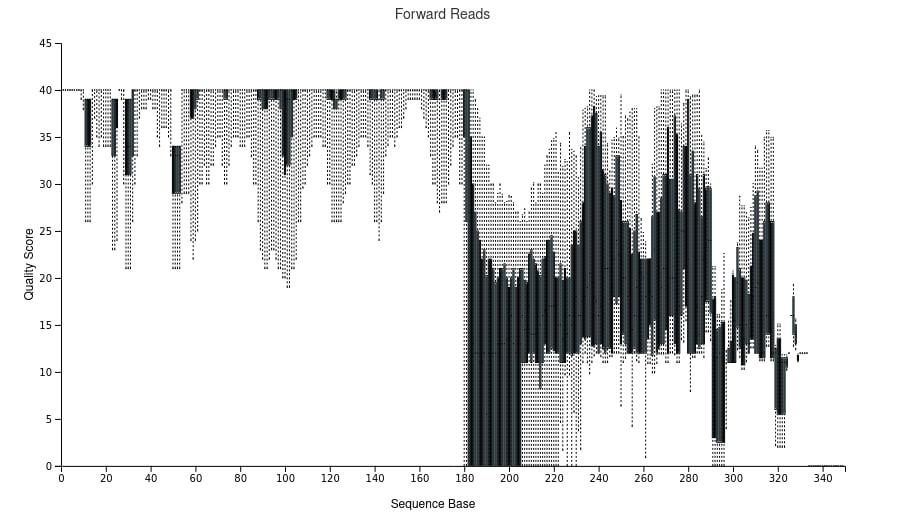
\includegraphics[scale=0.77]{1}  
	\caption{Quality Plot by QIIME2.}
	\label{heatmap1}
\end{figure}

Results and discussion will be divided by 2 parts ,as it follows from different data used,i.e. amplicon sequencing results and shotgun sequencing results. We will start from amplicon sequencing.
FastQC and visualization of seqs.qvz file clearly demonstrated us quality loss after postion of 180 bp, as also presence of untrimmed primer with UMI (see Fig.\ref{heatmap1} for hands-on proof). Based on supplementary data from SRA describing methods used to sequencing,we calculated total length of positions needed trimming (30: 21 bp primer+ 9 bp barcode). total length of reads after using DADA2 algorithm was bout of 150bp for each read. After denoising and trimming, only $49\%$ and $27\%$ of reads from bone and calculus data set respectively are passed filtering. See Suppl.Table 1 for more detailed info.

\begin{figure} 
	\centering
	\subfloat[\centering All taxons]{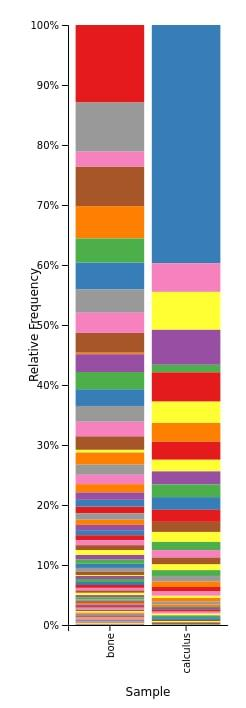
\includegraphics[scale=0.597]{2} }%
	\qquad
	\subfloat[\centering "red complex" taxons]{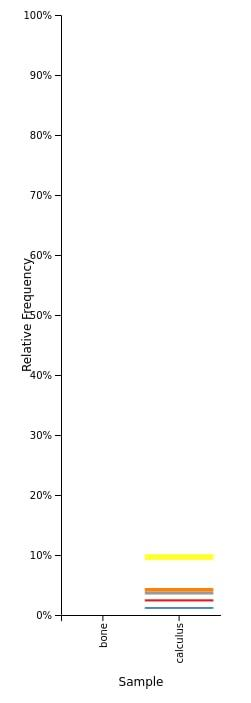
\includegraphics[scale=0.597]{3} }%
 
	\caption{Taxons. See legend for Fig. \ref{sup}.}%
	\label{fig:example}%
\end{figure}

  
 After constructing of feature table and mapping features IDs to sequences with BLAST we found 163 features with 5372 and 4781 frequency counts for bone and calculus samples respectively. taxonomic analysis was conducted with help of pre-trained Naive Bayes classifier GreenGenes(v.2020.2). Fig.\ref{fig:example} represents bar plot for taxonomy results, showing us whole little ecosystem consists of plethora of bacterial species. But out interest is more specific than just staring at well-coloured bands, so we narrowed our focus to find species especially associated with periodontal disease. We successfully detected presence of so-called "red complex" bacteria (see Fig.\ref{fig:example}),which are responsible for progression of various periodontal diseases. It clearly demonstrates that the same species involved in disease progression 1000 years and species described as suspects in 1998 are the same, thus partially verifying the main idea. One might ask "why we didn't find red complex in bone sample?'. Just because that these bacteria composing this complex prefer to live in specific conditions (i.e. acidity level, presence of another bacteria species etc), such as calculus--calcified dental plaque. So our findings looks legit and logical. To completely prove the idea, researchs had to preform the opposite taks--compare modern data with ancient. So begins our second part--shotgun sequencing and data analysis.

 

Person (ID G12) was selected for a dental calculus whole metagenome shotgun sequencing. After sequencing and assembling(assmebly part were skipped due to lack of computational resources) data were aligned vs MetaPhlAn database of human microbiota markers. Comparing our results with another set of samples taken from Human Microbiome Projetc(HMP) (See Suppl.Table 2 to find more info about accession and niche from which data were isolated) to better understanding of species abundance and taxonomy across our sample and HMP samples. To provide fancy heatmap for ease of reading and making right conclusions, hclust2 tool was used based on profiles samples and provided scores for species abundance. See Fig.\ref{heatmap4} for result of MetaPhlAn work.  Don't be afraid of black void scattered across this plot--it just means that this species just absent in one or more samples, which is normal. Moreover, if we suddenly find any of fecal bacteria or species descended from cervix inside dental calculus sample, it means BIG OOF by any means. Back to serious business. No doubt that G12 sample is the closest 'neighbour' for supragingival sample from HMP, seems OK. Intersections looks good--Rothia dentocariosa and Corynebacterium matruchotii(normal components of oral microbiomme). Other sampleshave almost no intarsection between each other, and it is also OK. Taxa abundance may(and even can) be different between petrified plaque and buccal mucosa, which cells are constantly renewing, as also from the nose, as also results from cervix and stool should differ entirely.

\begin{figure}[h]
	\centering
	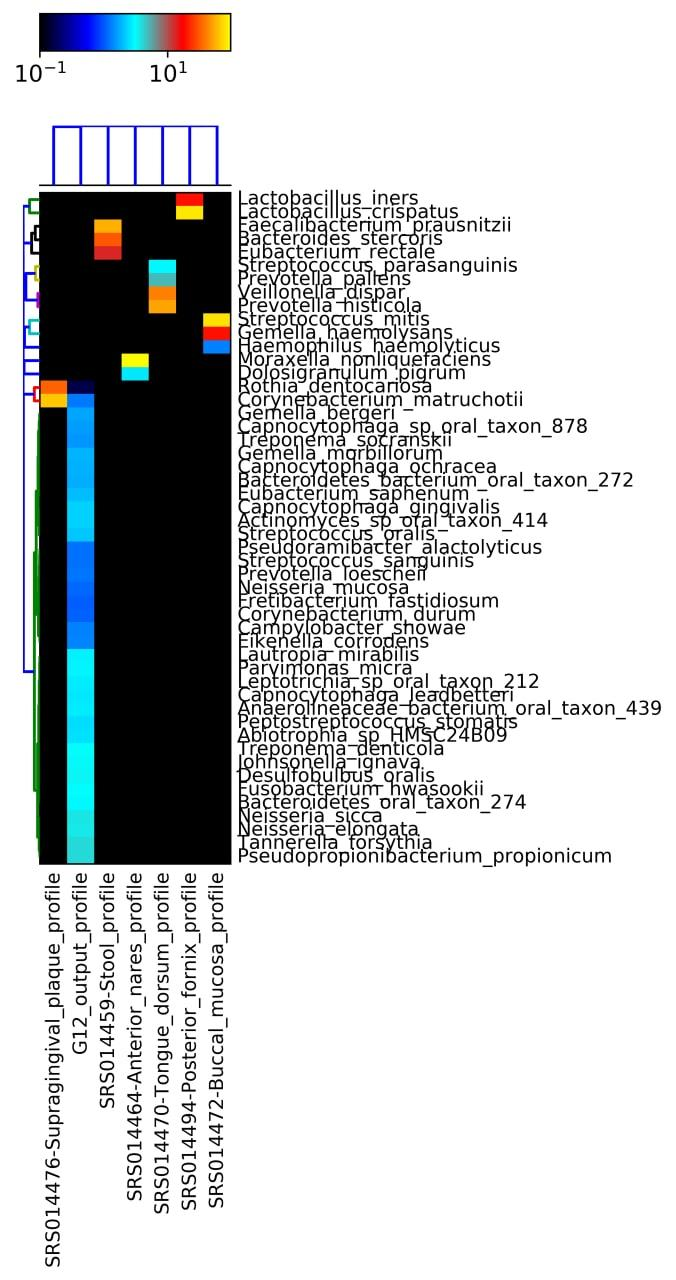
\includegraphics[scale=2.747]{4}  
	\caption{ Heatmap of distances between samples  }
	\label{heatmap4}
\end{figure}  
One more thing to do is to do the opposite thing from 1st part--perform comparison of modern samples with ancient Tannerella forsythia genome data. Using simpe pipeline (bwa$\rightarrow$samtools$\rightarrow$bedtools intersect) we obtained only intersecting regions between ancient and modern data, reducing results to only 388 entries, allowing us to just eye-balling the data. To put in simple,modern problems(such as dental health care) requires evolution. Not all of entries explain evolutionary mechanisms,some of them are ust 'hypothetical protein', but other findings clearly demonstrate adaptation to the changing environment. One of them is lanthionine synthetase C family protein which is member of group of peptide-modifying enzymes,for example, subtilin biosynthesis protein SpaC from Bacillus subtilis \cite{1}. Another example is IS1595-like element ISTfo1 family transposase(and other transposases found across entries list,such as IS1380 family transposase and IS4-like element IS421 family transposase), which is, like other transposases reposnible for gene transfer and rearrangements. We also found the presence of AIRP proteins, which are an abortive infection phage resistance proteins; they often found in restriction modification system operons, as described in \cite{2}. Some of the proteins are altered, e.g. GNAT family N-acetyltransferase which are participants in cell wall components syntheisis.Also we detected minor tweaks in metabolism, e.g. dihydrofolate reductase family proteins, beta-ketoacyl-ACP synthase III. Moreover, we found tetracycline resistance ribosomal protection protein, which is responsible for ... resistance, and here things get rough. Antibiotic resistance is a major problem threatening patients and doctors across the whole world. Taken into account that antibiotis are in use less than a century, this finding is clearly a new addition to the genome, and possibly it was added to the genome via HGT(horizontal gene transfer) medaited by transposases. We are sure that further investigation will provide more results, but it would take extensive amount of time,so we described here only most interesting cases. Unfortunately, we are unable to clearly find exact proteins, only families is known for our findings. We suggest that improved annotation will fix this problem.


And,the most pleasant part--final words and thoughts. I am actually surprised by effectiveness of modern bioinformatics methods allowing us to dig deeper and deeper. Yes, people from Middle Ages suffered from the same dental diseases. Algorithms working as they should, so no strange clustering occurred. Reversing this experiment gave us enough data to confirm presence of evolutional adaptions to new conditions by using rearrangements provided by transposases.This was one of my most favourite projects across the course.


Thank you for your attention!








\section{Supplement}

 
\begin{table}[h!]
	\centering
	\begin{tabular}{|c|c|}
		\hline
HMP_accession &	Niche   \\
\hline
SRS014459&	Stool 	   \\
\hline
SRS014464 &	Anterior_nares 	   \\
\hline
SRS014470 &	Tongue_dorsum 	   \\
\hline
SRS014472 & 	Buccal_mucosa 	   \\
\hline
SRS014476 &	Supragingival_plaque 	   \\
\hline 
SRS014494 &	Posterior_fornix \\ 
  	\hline	 

\end{tabular}
\caption{  Taxons }
\label{tab:var}
\end{table}

 \begin{figure}[h]
 	\centering
 	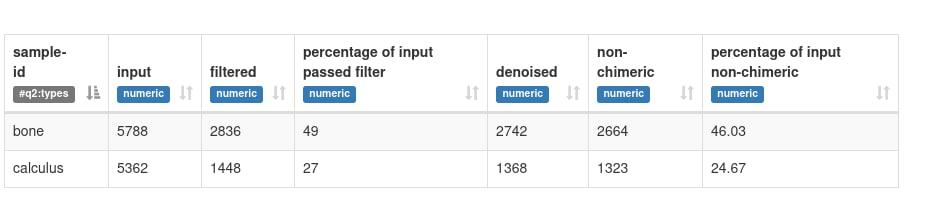
\includegraphics[scale=0.77]{supple}  
 	\caption{Supplement. 1. }
 	\label{heatmap11}
 \end{figure}
 
 \begin{figure}[h]
 	\centering
 	
\includegraphics[scale=0.3547]{leg}  
 	\caption{Legend  }
 	\label{sup}
 \end{figure} 
%\newpage 
%\newpage 
\begin{thebibliography}{9}



\bibitem{Data}
Raiko, Mike (2020): "Dead man's teeth" dataset. figshare. Dataset. https://doi.org/10.6084/m9.figshare.12152040.v3 


\bibitem{DataResearch}
	 Warinner, C., Rodrigues, J., Vyas, R. et al. Pathogens and host immunity in the ancient human oral cavity. Nat Genet 46, 336–344 (2014). https://doi.org/10.1038/ng.2906
	
	
	\bibitem{quime}
	Bolyen E, Rideout JR, Dillon MR, Bokulich NA, Abnet CC, Al-Ghalith GA, Alexander H, Alm EJ, Arumugam M, Asnicar F, Bai Y, Bisanz JE, Bittinger K, Brejnrod A, Brislawn CJ, Brown CT, Callahan BJ, Caraballo-Rodríguez AM, Chase J, Cope EK, Da Silva R, Diener C, Dorrestein PC, Douglas GM, Durall DM, Duvallet C, Edwardson CF, Ernst M, Estaki M, Fouquier J, Gauglitz JM, Gibbons SM, Gibson DL, Gonzalez A, Gorlick K, Guo J, Hillmann B, Holmes S, Holste H, Huttenhower C, Huttley GA, Janssen S, Jarmusch AK, Jiang L, Kaehler BD, Kang KB, Keefe CR, Keim P, Kelley ST, Knights D, Koester I, Kosciolek T, Kreps J, Langille MGI, Lee J, Ley R, Liu YX, Loftfield E, Lozupone C, Maher M, Marotz C, Martin BD, McDonald D, McIver LJ, Melnik AV, Metcalf JL, Morgan SC, Morton JT, Naimey AT, Navas-Molina JA, Nothias LF, Orchanian SB, Pearson T, Peoples SL, Petras D, Preuss ML, Pruesse E, Rasmussen LB, Rivers A, Robeson MS, Rosenthal P, Segata N, Shaffer M, Shiffer A, Sinha R, Song SJ, Spear JR, Swafford AD, Thompson LR, Torres PJ, Trinh P, Tripathi A, Turnbaugh PJ, Ul-Hasan S, van der Hooft JJJ, Vargas F, Vázquez-Baeza Y, Vogtmann E, von Hippel M, Walters W, Wan Y, Wang M, Warren J, Weber KC, Williamson CHD, Willis AD, Xu ZZ, Zaneveld JR, Zhang Y, Zhu Q, Knight R, and Caporaso JG. 2019. Reproducible, interactive, scalable and extensible microbiome data science using QIIME 2. Nature Biotechnology 37: 852–857. https://doi.org/10.1038/s41587-019-0209-9 
	
	
	\bibitem{Green}
	McDonald, D., Price, M., Goodrich, J. et al. An improved Greengenes taxonomy with explicit ranks for ecological and evolutionary analyses of bacteria and archaea. ISME J 6, 610–618 (2012). https://doi.org/10.1038/ismej.2011.139
	
	\bibitem{Met}
Integrating taxonomic, functional, and strain-level profiling of diverse microbial communities with bioBakery 3 Francesco Beghini, Lauren J McIver, Aitor Blanco-Miguez, Leonard Dubois, Francesco Asnicar, Sagun Maharjan, Ana Mailyan, Andrew Maltez Thomas, Paolo Manghi, Mireia Valles-Colomer, George Weingart, Yancong Zhang, Moreno Zolfo, Curtis Huttenhower, Eric A Franzosa, Nicola Segata. bioRxiv preprint (2020)
	
	
	\bibitem{BC}
	Bray, J. R. and J. T. Curtis. 1957. An ordination of upland forest communities of southern Wisconsin. Ecological Monographs 27:325-349.
	
	
	
	\bibitem{1}
	The subtilin gene of Bacillus subtilis ATCC 6633 is encoded in an operon that contains a homolog of the hemolysin B transport protein. Chung YJ, Steen MT, Hansen JN. J. Bacteriol. 174, 1417-22, (1992)
	
	\bibitem{2}
	 Iyer LM, Abhiman S, Aravind L; , Biol Direct. 2008;3:8.: MutL homologs in restriction-modification systems and the origin of eukaryotic MORC ATPases
	
	
\end{thebibliography}

 


\end{document}


